\documentclass[serif]{beamer}
%\usepackage[utopia]{mathdesign}
%\usepackage[no-math]{fontspec}
%\setmainfont{Liberation Serif}

\usepackage{minted}
\usepackage{hyperref}
\usepackage{ccicons}

\title{Python Numba for scientific code}
\author{Zbigniew Jędrzejewski-Szmek}
\institute{%
  %\includegraphics{beamer-themeredhat/redhat.png}\\
  \medskip
  \textit{zbyszek@in.waw.pl}\\
  \medskip
  \ccbysa
}
\date{\tiny Instytut im.\ M.\ Nęckiego, 25.11.2018}

\beamertemplatenavigationsymbolsempty

\addtobeamertemplate{navigation symbols}{}{%
    \usebeamerfont{footline}%
    \usebeamercolor[fg]{footline}%
    \hspace{1em}%
    \insertframenumber/\inserttotalframenumber
}

%% Pure Python code is too slow for many use cases, in particular
%% scientific and numerical calculations. The usual answer is to use
%% compiled code for parts of the program: either through libraries like
%% Numpy and BLAS, or through compiled Python extensions written in
%% Cython, a mix of C and Python.  A third option has become available —
%% machine code generated directly from the Python sources, using
%% just-in-time compilation. In lucky cases, this provides speed
%% comparable with optimized code in Cython or C, with the sources still
%% being pure Python.

\begin{document}
\begin{frame}
\titlepage % Print the title page as the first slide
\end{frame}

\begin{frame}
  \frametitle{Programmer time vs. computer time}
  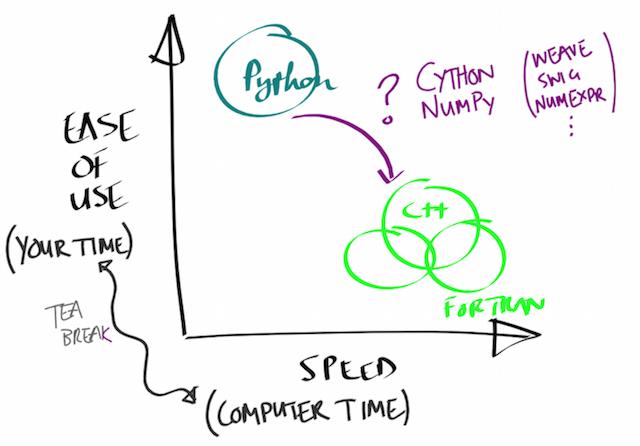
\includegraphics[width=\textwidth]{whycython.png}
\end{frame}

\begin{frame}
  \frametitle{Previous approaches}
  \framesubtitle{a.k.a. the graveyard of technologies}

  \begin{enumerate}
  \item Use compiled C or C++ or Fortran code with cpython
    \begin{itemize}
    \item C extension
    \item .so library + ctypes
    \item Fortran + f2py
    \item boost-python
    \item SWIG
    \item (Cython)
    \end{itemize}
    \pause
  \item A different Python interpreter
    \begin{itemize}
    \item jython
    \item psyco
    \item pypy
    \end{itemize}
    \pause

  \item Vectorization (numpy)
    \pause

  \item ``jit'' just the inner loop
    \begin{itemize}
    \item weave (Python + annotations to C++, inline)
    \item pyrex (Python + annotations to C, external)
    \item cython
    \item numexpr (``jitting'' of basic numpy array operations)
    \item numba
    \end{itemize}

  \end{enumerate}
\end{frame}

\begin{frame}[fragile,t]
  \frametitle{Special syntax}
  \framesubtitle{numexpr}

  \inputminted{python3}{numexpr_evaluate.py}
\end{frame}

\begin{frame}[fragile,t]
  \frametitle{Special syntax and type annotations}
  \framesubtitle{cython}

  \inputminted{python3}{cython_integrate.pyx}
\end{frame}

\begin{frame}[fragile,t]
  \frametitle{``jit''?}

  \begin{minted}{pycon}
>>> import numba

>>> @numba.jit
... def f(x):
...     y = x*5 + x
...     return y
  \end{minted}

  \pause
  \begin{minted}{pycon}
>>> f(1)
6
  \end{minted}
\end{frame}

\begin{frame}[fragile,t]
  \frametitle{\phantom{N}}

  \begin{minted}{pycon}
>>> import numpy as np
>>> x = np.eye(3)
>>> print('x:', x)
x: [[1. 0. 0.]
 [0. 1. 0.]
 [0. 0. 1.]]
>>> print('f(x):', f(x))
f(x): [[6. 0. 0.]
 [0. 6. 0.]
 [0. 0. 6.]]
  \end{minted}
  \pause
  \begin{minted}{pycon}
>>> f('abc')
'abcabcabcabcabcabc'
  \end{minted}
\end{frame}

\begin{frame}[fragile,t]
  \frametitle{\phantom{N}}
  \begin{minted}{pycon}
>>> f
CPUDispatcher(<function f at 0x...>)
>>> f.signatures
[(int64,),
 (array(float64, 2d, C),),
 (str,)]
>>> f.nopython_signatures
[(int64,) -> int64,
 (array(float64, 2d, C),) -> array(float64, 2d, C)]
  \end{minted}
\end{frame}

\begin{frame}
  \frametitle{Numba architecture}
  \hspace{-1cm}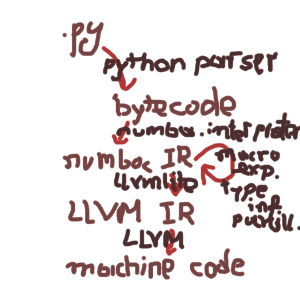
\includegraphics[width=0.8\textwidth]{numba_architecture.png}
\end{frame}

\begin{frame}[fragile,t]
  \frametitle{Some timings}

  \begin{minted}{python3}
def runningsum_loop(N):
    s = 0
    for i in range(N + 1):
        s += i
    return s
  \end{minted}
  \begin{minted}{text}
% timeit runningsum_loop(1_000_000)
54 ms ± 973 µs per loop (mean ± std. dev. of 7 runs,
                                       10 loops each)
  \end{minted}
\end{frame}

\begin{frame}[fragile,t]
  \frametitle{\phantom{S}}
  \begin{minted}{python3}
def runningsum_list(N):
    return sum([i for i in range(N + 1)])
  \end{minted}
  \begin{minted}{text}
%timeit runningsum_list(1_000_000)
52.7 ms ± 543 µs per loop (mean ± std. dev. of 7 runs,
                                        10 loops each)
  \end{minted}

  \pause

  \begin{minted}{python3}
def runningsum_generator(N):
    return sum(i for i in range(N + 1))
  \end{minted}
  \begin{minted}{text}
%timeit runningsum_generator(1_000_000)
50.4 ms ± 1.32 ms per loop (mean ± std. dev. of 7 runs,
                                         10 loops each)
  \end{minted}
\end{frame}

\begin{frame}[fragile,t]
  \frametitle{\phantom{S}}
  \begin{minted}{python3}
def runningsum_numpy(N):
    return np.arange(N+1).sum()
  \end{minted}
  \begin{minted}{text}
%timeit runningsum_numpy(1_000_000)
1.41 ms ± 76.8 µs per loop (mean ± std. dev. of 7 runs,
                                        1000 loops each)
  \end{minted}
\end{frame}

\begin{frame}[fragile,t]
  \frametitle{\phantom{S}}
  \begin{minted}{python3}
import numba

@numba.jit
def runningsum_numba_loop(N):
    s = 0
    for i in range(N + 1):
        s += i
    return s
  \end{minted}
  \pause
  \begin{minted}{text}
%timeit -r 1 -n 1 runningsum_numba_loop(1_000_000)
173 ms ± 0 ns per loop (mean ± std. dev. of 1 run,
                                       1 loop each)
  \end{minted}
  \pause
  \begin{minted}{text}
%timeit runningsum_numba_loop(1_000_000)
195 ns ± 5.48 ns per loop (mean ± std. dev. of 7 runs,
                                 10_000_000 loops each)
  \end{minted}
\end{frame}

\begin{frame}[fragile,t]
  \frametitle{\phantom{S}}
  \begin{minted}{C}
long int sum(int N) {
        long int s = 0;
        for (int i=0; i <= N; i++)
                s += i;
        return s;
}
int main(int argc, char **argv) {
        long int s;
        for (int i = 0; i < 10000; i++)
                s = sum(1000000);
        printf("%ld\n", s);
        return 0;
}
  \end{minted}
  \texttt{gcc -g -Wall} → 2.8 ms\\
  \texttt{gcc -g -Wall -O3} → \textless 1 µs (naive)\\
  \texttt{gcc -g -Wall -O3} → 237 µs (external compilation unit)
\end{frame}

\begin{frame}[fragile]
  \frametitle{Some timings — summary}

  \begin{tabular}{lrl}
    & time / ms\hspace{-0.5cm} \\
    \hline
    \texttt{runningsum\_loop} &    54 \\
    \texttt{runningsum\_list} &      53 \\
    \texttt{runningsum\_generator} &    50 \\
    \texttt{runningsum\_numpy} &   1.41 \\
    \texttt{runningsum\_numba\_loop} & 173 & (single iteration)\\
    \texttt{runningsum\_numba\_loop} & 0.000195 & (repeated) \\
    \texttt{runningsum\_c} & 2.8        & \texttt{-O0} \\
    \texttt{runningsum\_c} & \textless 0.001 & \texttt{-O3} \\
    \texttt{runningsum\_c} & 0.237 & \texttt{-O3},\\
    & & seperate compilation units
  \end{tabular}
\end{frame}

\begin{frame}[c]
  \Huge{Other numba features}
\end{frame}

\begin{frame}[fragile]
  \frametitle{Automatic parallelization}

  \begin{minted}{python}
def trig_ident_np(x):
    return (np.sin(x)**2 + np.cos(x)**2 +
            np.sin(x)**2 + np.cos(x)**2 +
            np.sin(x)**2 + np.cos(x)**2 +
            np.sin(x)**2 + np.cos(x)**2).sum()/4
  \end{minted}
  \pause
  \begin{minted}{python}
trig_ident_jit = numba.jit(trig_ident_np)
trig_ident_jitp = numba.jit(parallel=True)(trig_ident_np)
  \end{minted}
  \medskip
  \pause
  \begin{minted}{python}
x = np.random.randn(500, 50_000)
  \end{minted}
  \begin{minted}{text}
%timeit trig_ident_np(x)
4.52 s ± 160 ms per loop

%timeit trig_ident_jit(x)
788 ms ± 24 ms per loop

%timeit trig_ident_jitp(x)
290 ms ± 7.38 ms per loop
  \end{minted}
\end{frame}

\begin{frame}
  \frametitle{Hardware support}

  \begin{itemize}
  \item vector instructions (when CPU supports SSE, AVX, or AVX-512)
  \item Nvidia CUDA backend
  \end{itemize}
\end{frame}

\begin{frame}
  \frametitle{Evaluation of numba}

 \begin{itemize}
 \item good: native syntax and seamless integration
 \item good: excellent speed (when it works)
 \item bad: requires the whole LLVM backend to be present
 \item bad: hard to debug
 \item bad: not ``reproducible''
 \end{itemize}
\end{frame}

\begin{frame}[c]
  \Huge{Where is this all going?}
\end{frame}

\begin{frame}[fragile]
  \frametitle{Is Python a statically typed language?}

  \pause

  \inputminted{python3}{adder.py}

  \pause
  \begin{minted}{console}
$ mypy adder.py
adder.py:6: error: Argument 1 to "add" has incompatible
                   type "float"; expected "int"
adder.py:6: error: Argument 2 to "add" has incompatible
                   type "float"; expected "int"
  \end{minted}
\end{frame}

\begin{frame}
  \frametitle{The future?}

  \begin{itemize}
  \item Python continues to be used a glue language
  \item Python code is seamlessly compiled with various backends
  \item Type hints are used where automatic type inference is insufficient
  \end{itemize}
\end{frame}

\begin{frame}[fragile]
  \textcolor{gray}{The End}

  \bigskip

  %% \url{https://github.com/systemd/systemd}\\
  %% docs: \url{http://systemd.github.io/}\\
  %% \phantom{docs: }\url{https://www.freedesktop.org/wiki/Software/systemd/}\hspace*{-5cm}\\
  %% this: \url{https://github.com/keszybz/jesien-systemd-security}\hspace*{-5cm}
  %% \phantom{this: }\\
  %% \href{https://github.com/keszybz/jesien-systemd-security/blob/master/jesie%C5%84-systemd-security.pdf}{https://github.com/keszybz/jesien-systemd-security/blob/master/jesień-systemd-security.pdf}\hspace*{-5cm}
\end{frame}

\begin{frame}[fragile]
  \frametitle{Inspecting numba outputs}

  \begin{minted}{python3}
print(runningsum_numba_loop.inspect_llvm()[(numba.int64,)])
  \end{minted}
  \tiny
  \inputminted{llvm}{inspect_llvm.txt}
\end{frame}

\begin{frame}[fragile]
  \frametitle{Inspecting numba outputs}

  \begin{minted}{python3}
print(runningsum_numba_loop.inspect_asm()[(numba.int64,)])
  \end{minted}
  \tiny
  \inputminted{asm}{inspect_asm.txt}
\end{frame}

\end{document}
